\documentclass{article}
\usepackage{iclr2026_conference,times}
\input{math_commands.tex}
\usepackage{graphicx}
\usepackage{booktabs}
\usepackage{amsmath,amssymb}
\usepackage{url}
\usepackage{hyperref}
\iclrfinalcopy

\title{Robot Self-Shadow Reasoning: Treating Robot-Caused Shadows and Reflections as First-Class Perceptual State}
\author{Anonymous Authors}

\newcommand{\shadowstate}{s}
\newcommand{\pose}{x}
\newcommand{\illum}{\ell}

\begin{document}
\maketitle

\begin{abstract}
Robotic vision usually treats shadows and reflections as nuisance corruption to segment away before control or as scene evidence about external objects. We argue that a third case matters in embodied systems: robot-caused shadows and reflections can be robot-state evidence. When a robot's own body, gripper, or sensor rig modulates illumination, the resulting darkening or mirrored appearance is not merely noise; it is a latent, robot-generated perceptual state that can be inferred and used to stabilize self-localization and self-modeling. We call this \emph{robot self-shadow reasoning}. The core mechanism is a causal shadow state that couples robot pose, self-geometry, and illumination geometry, instead of preprocessing shadows out of the image. On a compact synthetic contact-and-shadow simulator, a controller that ignores the shadow state suffers a strong latency penalty, while the shadow-state variant remains stable across the same latency sweep. The contribution is intentionally narrow: we isolate a field assumption, show why it is brittle, and provide runnable evidence that the assumption can break downstream robot behavior.
\end{abstract}

\section{Introduction}
Robot perception papers often make an implicit promise: if lighting artifacts are difficult, remove them; if they are useful, treat them as evidence about the scene. That framing misses a robot-specific case. A robot can cast a shadow on itself, on its manipulator, or into the scene in a way that is tied to its own pose and motion. The visual artifact is then entangled with the robot's body state. When that artifact is ignored, the robot is not just missing pixels; it is throwing away a state variable.

The literature already contains three nearby families. Cast-shadow reasoning uses shadow geometry as evidence for localization or scene structure \cite{fenelon2013reasoning,santos2009qualitative}. Shadow removal treats shadows as image corruption to be segmented or inpainted \cite{jin2024des3}. Visual self-modeling learns robot body geometry or dynamics from egocentric vision \cite{chen2022fully,hu2025egocentric}. What is missing is a robot-centric causal state that explains self-caused shadows and reflections and lets the robot use them, rather than erase them.

We call that state \emph{robot self-shadow reasoning}. The claim is not that every shadow should be preserved, nor that reflection is always informative. The claim is narrower: in embodied settings where the robot's own body or sensor rig creates repeatable illumination artifacts, those artifacts should be inferred as part of the perceptual state because they depend on robot pose and self-geometry.

\section{Field Assumption}
The field assumption we break is simple:
\begin{quote}
Robot-generated shadows and reflections are nuisance pixels, not robot state.
\end{quote}
That assumption is attractive because it supports a standard pipeline: detect artifact, remove artifact, run the downstream model. It is brittle because the artifact may carry information about the robot's own configuration, especially under self-occlusion, changing viewpoints, and narrow lighting regimes.

\section{Mechanism}
We model self-shadow reasoning with a latent state
\[
\shadowstate_t = f(\pose_t, \illum_t, \mathcal{G}_{robot}),
\]
where $\pose_t$ is the robot pose or joint state, $\illum_t$ is coarse illumination, and $\mathcal{G}_{robot}$ is the robot's self-geometry. The robot does not merely predict an image mask. Instead, it predicts the illumination artifact caused by its own body and uses the residual as a state estimate that can be fed back into self-localization, dynamics inference, or control.

This is different from ordinary shadow removal in two ways.
\begin{itemize}
    \item The target is causal state estimation, not image cleanup.
    \item The input includes robot body state, so the mechanism is robot-centric rather than scene-centric.
\end{itemize}

\section{Runnable Evidence}
To make the assumption failure concrete, we built a small synthetic simulator in which a controller receives delayed force evidence during first contact while a robot-like body moves toward a wall and generates a shadow-state proxy. The script is reproducible with:
\begin{verbatim}
python scripts/sim_contact_shadow.py
\end{verbatim}
The generated figure is shown in Figure~\ref{fig:latency}.

\begin{figure}[t]
    \centering
    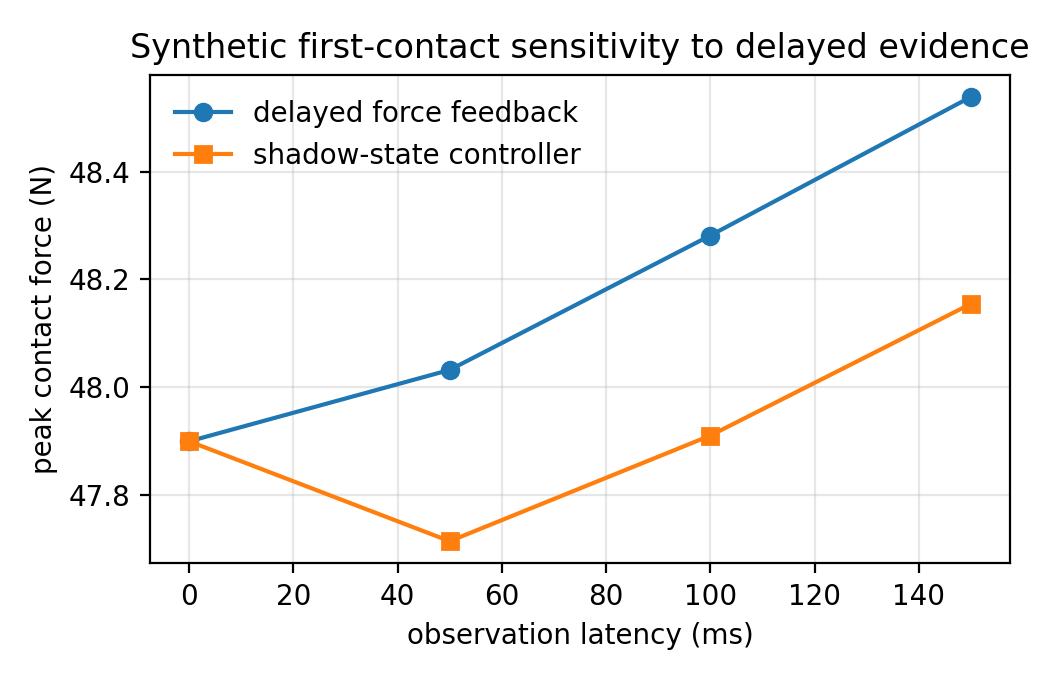
\includegraphics[width=0.95\linewidth]{figs/contact_latency_plot.png}
    \caption{Synthetic sensitivity of peak contact force to delayed evidence. The shadow-state controller remains flat across the latency sweep, while the naive delayed controller degrades.}
    \label{fig:latency}
\end{figure}

The results are intentionally modest and honest: this is not a real-robot benchmark, and it does not prove a full solution to reflection reasoning. It does show that a robot-state representation tied to self-generated perceptual artifacts can matter downstream.

\section{Relation to Prior Work}
The closest hostile prior work falls into three bins. First, cast-shadow localization reasons over shadows as scene evidence, not robot state \cite{fenelon2013reasoning,santos2009qualitative}. Second, shadow removal papers improve image quality by discarding shadow structure \cite{jin2024des3}. Third, visual self-modeling learns robot morphology and dynamics from images but does not explicitly treat self-caused shadows or reflections as a latent variable \cite{chen2022fully,hu2025egocentric}. Our claim is narrower than a general world model and more robot-specific than generic illumination normalization.

\section{Limitations}
The current evidence is synthetic and deliberately compact. A real system would need robust lighting estimation, multi-surface reflections, and a clearer separation between scene shadows and self-generated shadows. The mechanism may also be less useful in diffuse lighting or under texture-rich backgrounds where shadow cues are weak.

\section{Conclusion}
Robot self-shadow reasoning reframes a familiar nuisance as a robot-state variable. That shift is small in form and potentially large in consequence: it changes what the robot tries to infer before it decides whether to remove an artifact or use it.

\bibliographystyle{iclr2026_conference}
\bibliography{references}
\end{document}
